\section{Recurrent Neural Network Based Occupancy Estimation}
\label{sec:rnn-method}

In this section, we apply the Elman's recurrent neural network (ELNN) architecture shown in
Fig.~\ref{fig:elman} to the occupancy of each room in a certain smart building.
We describe the ELNN structure, how the gold-referencing data is
computed, and the detailed works on training the networks. ELNN architecture is used to build the black-box model for occupancy estimation. In this case the size (number of neurons) of hidden layers are assigned according
to the empirical equation $N_{1,\ldots,k-1}=\frac15p+5$ and $N_k=2q$, where $N_i$
is the size of $i$th layer, and $p$ and $q$ are the number of network
inputs and outputs, respectively.

\begin{figure}[t]
    \centering
    \includegraphics[width=0.9\columnwidth]{figs/rnn/elman}
    \caption{Architecture of Elman Recurrent Neural Network}
    \label{fig:elman}
\end{figure}

\EP{} takes outdoor thermal factors (such as ambient temperatures and solar
factors), people occupancy and HVAC related powers as input, and produce the
temperatures of rooms as it's output. People occupancy is in unit of number of
people, which maybe decimal as it represents average people count over a short
time span. We treat all the data used and produced by \EP{} equally as
real-world factors, regardless they were inputs or outputs of \EP{}. In the
occupancy estimation work, we select data from those real-world factors, feed
them into the recurrent neural network, and try to get estimated occupancy from
it.

We use \EP{} to simulate the room thermal behavior in a year, using various
inputs including occupancy information. We collect the inputs and outputs (room
temperatures) of \EP{} simulation, which is discretized into hourly data
points, to train ELNN. Given the simulated data
provided by \EP{}, as shown in Fig.\ref{fig:data-flow}, we feed selected
channels of ambient factors and other power data, along with room temperatures,
into ELNN as input. We use estimated and real
occupancy to drive the training process. We will configure two different
selected datasets: one uses ambient factors and room temperatures only, another
dataset uses ambient factors, room temperatures and HVAC cooling/heating
powers. The output of ELNN has multiple channels, which are
respectively each room's estimated people occupancy.

\begin{figure}[t]
    \centering
    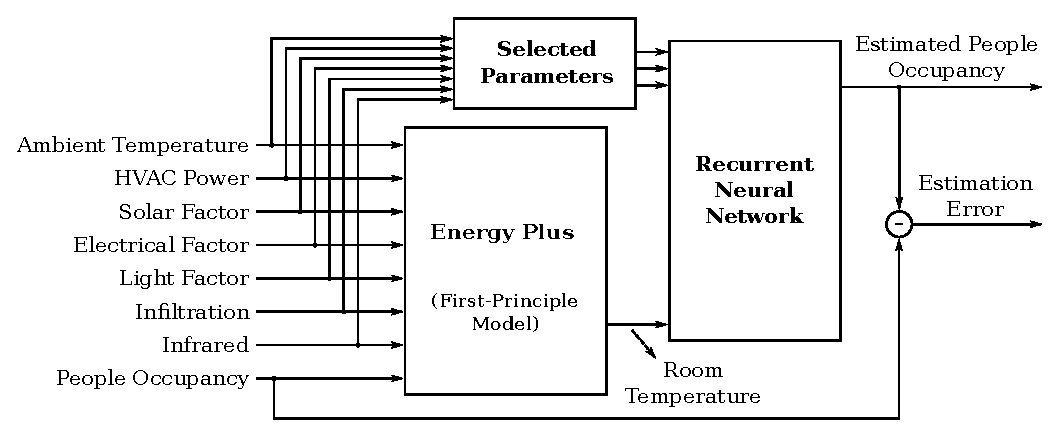
\includegraphics[width=0.9\columnwidth]{figs/rnn/data-flow.eps}
    \caption{Data configuration of Elman's recurrent neuron network.}
    \label{fig:data-flow}
\end{figure}

In practical smart-building applications, room temperatures are easy to acquire
from the installed sensors. Ambient temperature, solar factors are also
relatively easier to be acquired or calculated. While other factors, such as
HVAC colling or heating powers, electrical equipment powers and air
infiltrations, need more instruments to per-room estimate in real-time. Because
of these limitations, we select two different sets of real-world factors as the
network input and compare the occupancy evaluation accuracy.
\begin{enumerate}
    \item Input includes ambient temperature, solar factors and room
    temperatures only. This will be referred as configuration I from now on.

    \item Input includes ambient temperature, solar factors, room temperatures
    and HVAC cooling\slash{}heating powers. This will be referred as configuration II from now on.
\end{enumerate}
With different factors as network inputs, we also configure the recurrent
neural network with different hidden recurrent layers varying from one to
three ($k=1,2,3$), to compare the estimation accuracies. We divide the one year
simulation data into 12 months. Months 1--3, 5--7, 9--11 are used for training;
months 4, 8, 12 are used for validating the trained networks.

